% This is the Reed College LaTeX thesis template. Most of the work
% for the document class was done by Sam Noble (SN), as well as this
% template. Later comments etc. by Ben Salzberg (BTS). Additional
% restructuring and APA support by Jess Youngberg (JY).
% Your comments and suggestions are more than welcome; please email
% them to cus@reed.edu
%
% See https://www.reed.edu/cis/help/LaTeX/index.html for help. There are a
% great bunch of help pages there, with notes on
% getting started, bibtex, etc. Go there and read it if you're not
% already familiar with LaTeX.
%
% Any line that starts with a percent symbol is a comment.
% They won't show up in the document, and are useful for notes
% to yourself and explaining commands.
% Commenting also removes a line from the document;
% very handy for troubleshooting problems. -BTS

% As far as I know, this follows the requirements laid out in
% the 2002-2003 Senior Handbook. Ask a librarian to check the
% document before binding. -SN

%%
  %% Preamble
%%
  % \documentclass{<something>} must begin each LaTeX document
\documentclass[12pt,twoside]{smiththesis}
% Packages are extensions to the basic LaTeX functions. Whatever you
% want to typeset, there is probably a package out there for it.
% Chemistry (chemtex), screenplays, you name it.
% Check out CTAN to see: https://www.ctan.org/
  %%
  \usepackage{graphicx,latexsym}
\usepackage{amsmath}
\usepackage{amssymb,amsthm}
\usepackage{longtable,booktabs,setspace}
\usepackage{chemarr} %% Useful for one reaction arrow, useless if you're not a chem major
\usepackage[hyphens]{url}
% Added by CII
\usepackage{hyperref}
\usepackage{lmodern}
\usepackage{multicol}
\usepackage{float}
\floatplacement{figure}{H}
% End of CII addition
\usepackage{rotating}
%\hypersetup{
%    colorlinks=true,
%    linkcolor=blue,
%    filecolor=magenta,      
 %   urlcolor=blue,
 %   pdftitle={Overleaf Example},
 %   pdfpagemode=FullScreen,
 %   }

% Next line commented out by CII
%%% \usepackage{natbib}
% Comment out the natbib line above and uncomment the following two lines to use the new
% biblatex-chicago style, for Chicago A. Also make some changes at the end where the
% bibliography is included.
%\usepackage{biblatex-chicago}
%\bibliography{thesis}


% Added by CII (Thanks, Hadley!)
% Use ref for internal links
\renewcommand{\hyperref}[2][???]{\autoref{#1}}
\def\chapterautorefname{Chapter}
\def\sectionautorefname{Section}
\def\subsectionautorefname{Subsection}
% \hypersetup{
%     colorlinks=true,
%     linkcolor=blue,
%    filecolor=blue,
%     citecolor = blue,      
%     urlcolor=cyan,
 %    }
\hypersetup{colorlinks=true,
            linkcolor=blue,
            citecolor=black,
            urlcolor=blue}
% End of CII addition

% Added by CII
\usepackage{caption}
\captionsetup{width=5in}
% End of CII addition

% \usepackage{times} % other fonts are available like times, bookman, charter, palatino
\usepackage{palatino}
\usepackage{tcolorbox}

% Syntax highlighting #22

% To pass between YAML and LaTeX the dollar signs are added by CII
\title{Estimating Unobserved COVID-19 Infections in the United States}
\author{Quinn White}
% The month and year that you submit your FINAL draft TO THE LIBRARY (May or December)
\date{May 2023}
\division{Mathematics and Natural Sciences}
\advisor{Ben Baumer}
\institution{Smith College}
\degree{Bachelor of Arts}
%If you have two advisors for some reason, you can use the following
% Uncommented out by CII
\altadvisor{Nicholas Reich}
% End of CII addition

%%% Remember to use the correct department!
\department{Statistical and Data Sciences}
% if you're writing a thesis in an interdisciplinary major,
% uncomment the line below and change the text as appropriate.
% check the Senior Handbook if unsure.
%\thedivisionof{The Established Interdisciplinary Committee for}
% if you want the approval page to say "Approved for the Committee",
% uncomment the next line
%\approvedforthe{Committee}

% Added by CII
%%% Copied from knitr
%% maxwidth is the original width if it's less than linewidth
%% otherwise use linewidth (to make sure the graphics do not exceed the margin)
\makeatletter
\def\maxwidth{ %
  \ifdim\Gin@nat@width>\linewidth
    \linewidth
  \else
    \Gin@nat@width
  \fi
}
\makeatother

\renewcommand{\contentsname}{Table of Contents}
% End of CII addition

\setlength{\parskip}{0pt}

% Added by CII

\providecommand{\tightlist}{%
  \setlength{\itemsep}{0pt}\setlength{\parskip}{0pt}}

\Acknowledgements{
Will add
}

\Dedication{
You can have a dedication here if you wish.
}


\Abstract{
As we have navigated the COVID-19 pandemic, case counts have been a central source of information for understanding transmission dynamics and the effect of public health interventions. However, because the number of cases we observe is limited by the testing effort in a given location, the case counts presented on local or national dashboards are only a fraction of the true infections. Variations in testing rate by time and location impacts the number of cases that go unobserved, which can cloud our understanding of the true COVID-19 incidence at a given time point and can create biases in downstream analyses. Additionally, the number of cases we observe is impacted by the sensitivity and specificity of the diagnostic test. To quantify the number of true infections given incomplete testing and diagnostic test inaccuracy, this work implements probabilistic bias analysis at a biweekly time scale from January 1, 2021 through February 2022. In doing so, we can estimate a range of possible true infections for a given time interval and location. This approach can be applied at the state level across the United States, as well as in some counties where the needed data are available.
}

% End of CII addition
%%
%% End Preamble
%%
%
\begin{document}

% Everything below added by CII
  \maketitle

\frontmatter % this stuff will be roman-numbered
\pagestyle{empty} % this removes page numbers from the frontmatter
  \begin{acknowledgements}
    Will add
  \end{acknowledgements}

% https://github.com/ismayc/thesisdown/issues/32 
  {
    \hypersetup{linkcolor=black}
    \setcounter{tocdepth}{2}
    \tableofcontents
  }


  \begin{abstract}
    As we have navigated the COVID-19 pandemic, case counts have been a central source of information for understanding transmission dynamics and the effect of public health interventions. However, because the number of cases we observe is limited by the testing effort in a given location, the case counts presented on local or national dashboards are only a fraction of the true infections. Variations in testing rate by time and location impacts the number of cases that go unobserved, which can cloud our understanding of the true COVID-19 incidence at a given time point and can create biases in downstream analyses. Additionally, the number of cases we observe is impacted by the sensitivity and specificity of the diagnostic test. To quantify the number of true infections given incomplete testing and diagnostic test inaccuracy, this work implements probabilistic bias analysis at a biweekly time scale from January 1, 2021 through February 2022. In doing so, we can estimate a range of possible true infections for a given time interval and location. This approach can be applied at the state level across the United States, as well as in some counties where the needed data are available.
  \end{abstract}
  \begin{dedication}
    You can have a dedication here if you wish.
  \end{dedication}
\mainmatter % here the regular arabic numbering starts
\pagestyle{fancyplain} % turns page numbering back on

\hypertarget{motivation}{%
\chapter{Motivation}\label{motivation}}

Placeholder

\hypertarget{background}{%
\chapter{Background}\label{background}}

Placeholder

\hypertarget{probabalistic-bias-analysis}{%
\section{Probabalistic Bias Analysis}\label{probabalistic-bias-analysis}}

\hypertarget{background-for-the-approach}{%
\section{Background for the Approach}\label{background-for-the-approach}}

\hypertarget{simple-discrete-example}{%
\subsection{Simple Discrete Example}\label{simple-discrete-example}}

\hypertarget{general-solution-for-the-discrete-case}{%
\subsection{General Solution for the Discrete Case}\label{general-solution-for-the-discrete-case}}

\hypertarget{general-solution-for-the-continuous-case}{%
\subsection{General Solution for the Continuous Case}\label{general-solution-for-the-continuous-case}}

\hypertarget{implementation-through-the-sampling-importance-resampling-algorithm}{%
\subsection{Implementation through the Sampling-Importance-Resampling Algorithm}\label{implementation-through-the-sampling-importance-resampling-algorithm}}

\hypertarget{bayesian-melding-applied-to-covid-19-misclassification}{%
\section{Bayesian Melding Applied to COVID-19 Misclassification}\label{bayesian-melding-applied-to-covid-19-misclassification}}

\hypertarget{distribution-of-theta-alpha-beta-ps_1textuntested}{%
\subsection{\texorpdfstring{Distribution of \(\theta = \{\alpha, \beta, P(S_1|\text{untested}) \}\)}{Distribution of \textbackslash theta = \textbackslash\{\textbackslash alpha, \textbackslash beta, P(S\_1\textbar\textbackslash text\{untested\}) \textbackslash\}}}\label{distribution-of-theta-alpha-beta-ps_1textuntested}}

\hypertarget{direct-prior-and-induced-prior-distributions-for-ps_0texttest_textuntested}{%
\subsection{\texorpdfstring{Direct Prior and Induced Prior Distributions for \(P(S_0|\text{test}_+,\text{untested})\)}{Direct Prior and Induced Prior Distributions for P(S\_0\textbar\textbackslash text\{test\}\_+,\textbackslash text\{untested\})}}\label{direct-prior-and-induced-prior-distributions-for-ps_0texttest_textuntested}}

\hypertarget{pooling}{%
\subsection{Pooling}\label{pooling}}

\hypertarget{derivation}{%
\subsection{\texorpdfstring{Derivation of \(M\)}{Derivation of M}}\label{derivation}}

\hypertarget{sampling-importance-resampling-algorithm}{%
\section{\texorpdfstring{Sampling-Importance-Resampling Algorithm \label{sampling}}{Sampling-Importance-Resampling Algorithm }}\label{sampling-importance-resampling-algorithm}}

\hypertarget{overview}{%
\subsection{Overview}\label{overview}}

\hypertarget{proof}{%
\subsection{Proof that Algorithm Obtains Approximate Sample from Target Distribution}\label{proof}}

\hypertarget{example-1}{%
\subsubsection{Example 1:}\label{example-1}}

\hypertarget{example-2}{%
\subsubsection{Example 2:}\label{example-2}}

\hypertarget{logpooled}{%
\subsection{Obtaining Logarithmic Pooled Distribution with the Sampling-Importance-Resampling Algorithm}\label{logpooled}}

\hypertarget{presamp}{%
\subsection{Implications of the Sample Size and Resample Size}\label{presamp}}

\hypertarget{loess-smoothing}{%
\section{LOESS Smoothing}\label{loess-smoothing}}

\hypertarget{introduction}{%
\subsection{Introduction}\label{introduction}}

\hypertarget{fitting-the-loess-curve}{%
\subsection{Fitting the LOESS Curve}\label{fitting-the-loess-curve}}

\hypertarget{kernel-density-estimation}{%
\section{Kernel Density Estimation}\label{kernel-density-estimation}}

\hypertarget{overview-1}{%
\subsection{Overview}\label{overview-1}}

\hypertarget{bounded-density-estimation}{%
\subsection{Bounded Density Estimation}\label{bounded-density-estimation}}

\hypertarget{definition-of-prior-distributions-for-bias-parameters}{%
\chapter{Definition of Prior Distributions for Bias Parameters}\label{definition-of-prior-distributions-for-bias-parameters}}

Placeholder

\hypertarget{background-on-the-beta-distribution}{%
\section{Background on the Beta Distribution}\label{background-on-the-beta-distribution}}

\hypertarget{background-on-the-gamma-distribution}{%
\section{Background on the Gamma Distribution}\label{background-on-the-gamma-distribution}}

\hypertarget{definition-of-prior-distributions-for-incomplete-testing-correction}{%
\section{Definition of Prior Distributions for Incomplete Testing Correction}\label{definition-of-prior-distributions-for-incomplete-testing-correction}}

\hypertarget{defining-ps_1untested}{%
\subsection{\texorpdfstring{Defining \(P(S_1|Untested)\)}{Defining P(S\_1\textbar Untested)}}\label{defining-ps_1untested}}

\hypertarget{defining-alpha}{%
\subsection{\texorpdfstring{Defining \(\alpha\)}{Defining \textbackslash alpha}}\label{defining-alpha}}

\hypertarget{defining-beta}{%
\subsection{\texorpdfstring{Defining \(\beta\)}{Defining \textbackslash beta}}\label{defining-beta}}

\hypertarget{defining-ps_0testuntested}{%
\subsection{\texorpdfstring{Defining \(P(S_0|test+,untested)\)}{Defining P(S\_0\textbar test+,untested)}}\label{defining-ps_0testuntested}}

\hypertarget{definition-of-priors-for-test-inaccuracy-correction}{%
\section{Definition of Priors for Test Inaccuracy Correction}\label{definition-of-priors-for-test-inaccuracy-correction}}

\hypertarget{defining-test-sensitivity-s_e}{%
\subsection{\texorpdfstring{Defining Test Sensitivity (\(S_e\))}{Defining Test Sensitivity (S\_e)}}\label{defining-test-sensitivity-s_e}}

\hypertarget{defining-test-specificity-s_p}{%
\section{\texorpdfstring{Defining Test Specificity (\(S_p\))}{Defining Test Specificity (S\_p)}}\label{defining-test-specificity-s_p}}

\hypertarget{summary-table-of-bias-parameter-distributions}{%
\section{Summary Table of Bias Parameter Distributions}\label{summary-table-of-bias-parameter-distributions}}

\hypertarget{correction-for-incomplete-testing}{%
\section{Correction for Incomplete Testing}\label{correction-for-incomplete-testing}}

\hypertarget{correction-for-diagnostic-test-inaccuracy}{%
\section{Correction for Diagnostic Test Inaccuracy}\label{correction-for-diagnostic-test-inaccuracy}}

\hypertarget{derivation-of-formula-for-correction-for-diagnostic-test-inaccuracy}{%
\subsection{Derivation of Formula for Correction for Diagnostic Test Inaccuracy}\label{derivation-of-formula-for-correction-for-diagnostic-test-inaccuracy}}

\hypertarget{details-of-implementation}{%
\chapter{Details of Implementation}\label{details-of-implementation}}
\begin{itemize}
\tightlist
\item
  Describe each step here
\item
  Mention reproducible workflow with make
\end{itemize}
\hypertarget{reproducible-workflow}{%
\section{Reproducible Workflow}\label{reproducible-workflow}}

\hypertarget{results}{%
\chapter{Results}\label{results}}

Placeholder

\hypertarget{county}{%
\section{County}\label{county}}

\hypertarget{state}{%
\section{State}\label{state}}

\hypertarget{comparison-to-the-covidestim-model}{%
\section{Comparison to the Covidestim Model}\label{comparison-to-the-covidestim-model}}

\hypertarget{overview-2}{%
\subsection{Overview}\label{overview-2}}

\hypertarget{the-covidestim-model}{%
\subsection{The Covidestim Model}\label{the-covidestim-model}}

\hypertarget{assumptions}{%
\subsection{Assumptions}\label{assumptions}}

\hypertarget{the-model}{%
\subsection{The Model}\label{the-model}}

\hypertarget{comparison-to-other-indicators}{%
\subsection{Comparison to Other Indicators}\label{comparison-to-other-indicators}}

\hypertarget{comparison-to-other-indicators-1}{%
\subsection{Comparison to Other Indicators}\label{comparison-to-other-indicators-1}}

\hypertarget{limitations-of-this-comparison}{%
\subsection{Limitations of this Comparison}\label{limitations-of-this-comparison}}

\hypertarget{seropositivity-data}{%
\section{Seropositivity Data}\label{seropositivity-data}}

\hypertarget{county-level}{%
\section{County-level}\label{county-level}}

\hypertarget{state-level}{%
\section{State-level}\label{state-level}}

\hypertarget{cross-correlation-comparison}{%
\section{Cross Correlation Comparison}\label{cross-correlation-comparison}}

\appendix

\hypertarget{appendix}{%
\chapter{Appendix}\label{appendix}}

\hypertarget{smoothing-span}{%
\section{Smoothing Span}\label{smoothing-span}}

\hypertarget{changing-span-for-loess-smoothing-of-beta}{%
\subsection{\texorpdfstring{Changing SPAN for LOESS Smoothing of \(\beta\)}{Changing SPAN for LOESS Smoothing of \textbackslash beta}}\label{changing-span-for-loess-smoothing-of-beta}}

\hypertarget{changing-mean-and-variance-for-prior-distribution-specifications}{%
\section{Changing Mean and Variance for Prior Distribution Specifications}\label{changing-mean-and-variance-for-prior-distribution-specifications}}

\hypertarget{relationship-between-xy_alpha-and-x_alpha-y_alpha-for-dependent-variables-xy}{%
\section{\texorpdfstring{Relationship Between \((X+Y)_\alpha\) and \(X_alpha\) +\(Y_\alpha\) for Dependent Variables \(X,Y\)}{Relationship Between (X+Y)\_\textbackslash alpha and X\_alpha +Y\_\textbackslash alpha for Dependent Variables X,Y}}\label{relationship-between-xy_alpha-and-x_alpha-y_alpha-for-dependent-variables-xy}}

\hypertarget{simulation-bivariate-normal}{%
\subsection{Simulation: Bivariate Normal}\label{simulation-bivariate-normal}}

We can see this in a concrete example. Let \((X,Y)\) be bivariate normal with \(\boldsymbol \mu = \begin{pmatrix} 0\\0\end{pmatrix}\) and correlation matrix \(\boldsymbol \Sigma = \begin{pmatrix} 1 & \rho \\ \rho & 1 \end{pmatrix}\), and hence where \(X, Y\) are marginally standard normal random variables.

We let the subscript \(\alpha\) denote the \(\alpha^{th}\) and the subscript \(1-\alpha\) denote the \((1-\alpha)^{th}\) quantile of the distribution.

In Figure \ref{fig:simmvn}, in each panel, we increase the correlation \(\rho\) between \(X\) and \(Y\) by 0.25 units and plot the sum \(X +Y\) against \(X\). The vertical lines represent quantiles \(X_{0.025}\) and \(X_{0.975}\), and the horizontal lines represent the quantiles \((X+Y)_{0.025}\) and \((X+Y)_{0.975}\).

We see in Figure \ref{fig:simmvn} that when we increase the correlation between \(X\) and \(Y\), the width of the interval \(\Big((X+Y)_\alpha, (X+Y)_{1-\alpha}\Big)\) increases.
\begin{figure}

{\centering 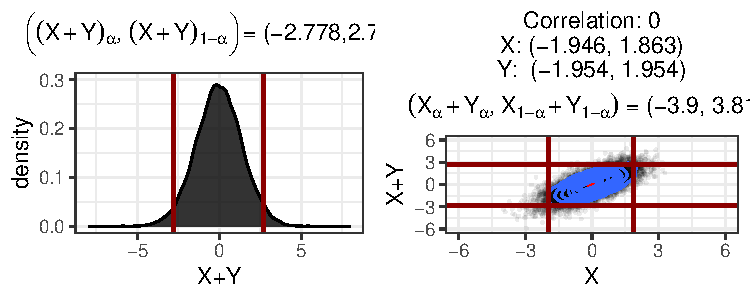
\includegraphics[width=0.96\linewidth]{thesis_files/figure-latex/unnamed-chunk-2-1} 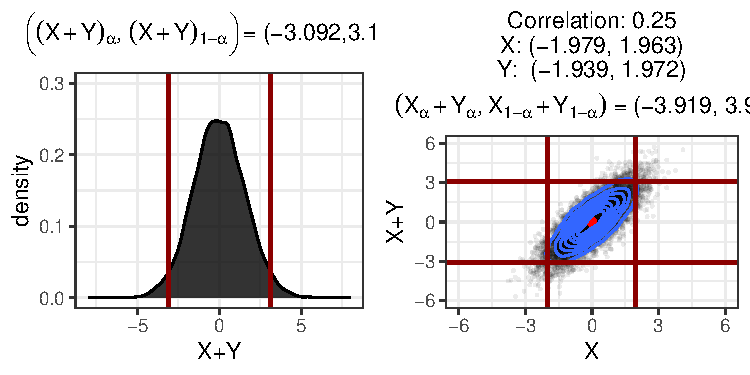
\includegraphics[width=0.96\linewidth]{thesis_files/figure-latex/unnamed-chunk-2-2} 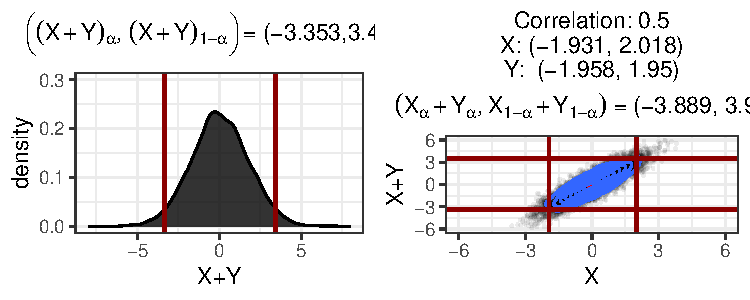
\includegraphics[width=0.96\linewidth]{thesis_files/figure-latex/unnamed-chunk-2-3} 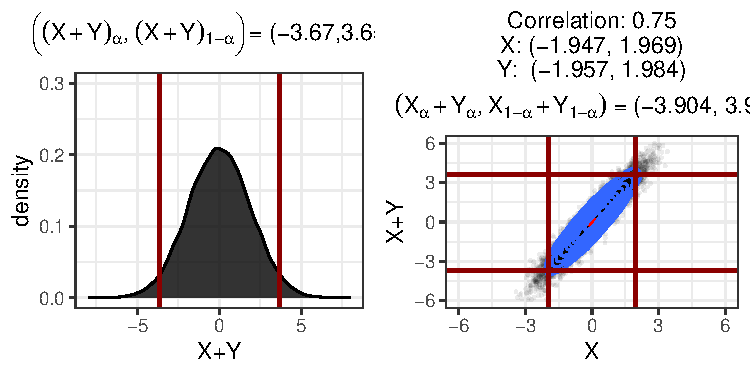
\includegraphics[width=0.96\linewidth]{thesis_files/figure-latex/unnamed-chunk-2-4} 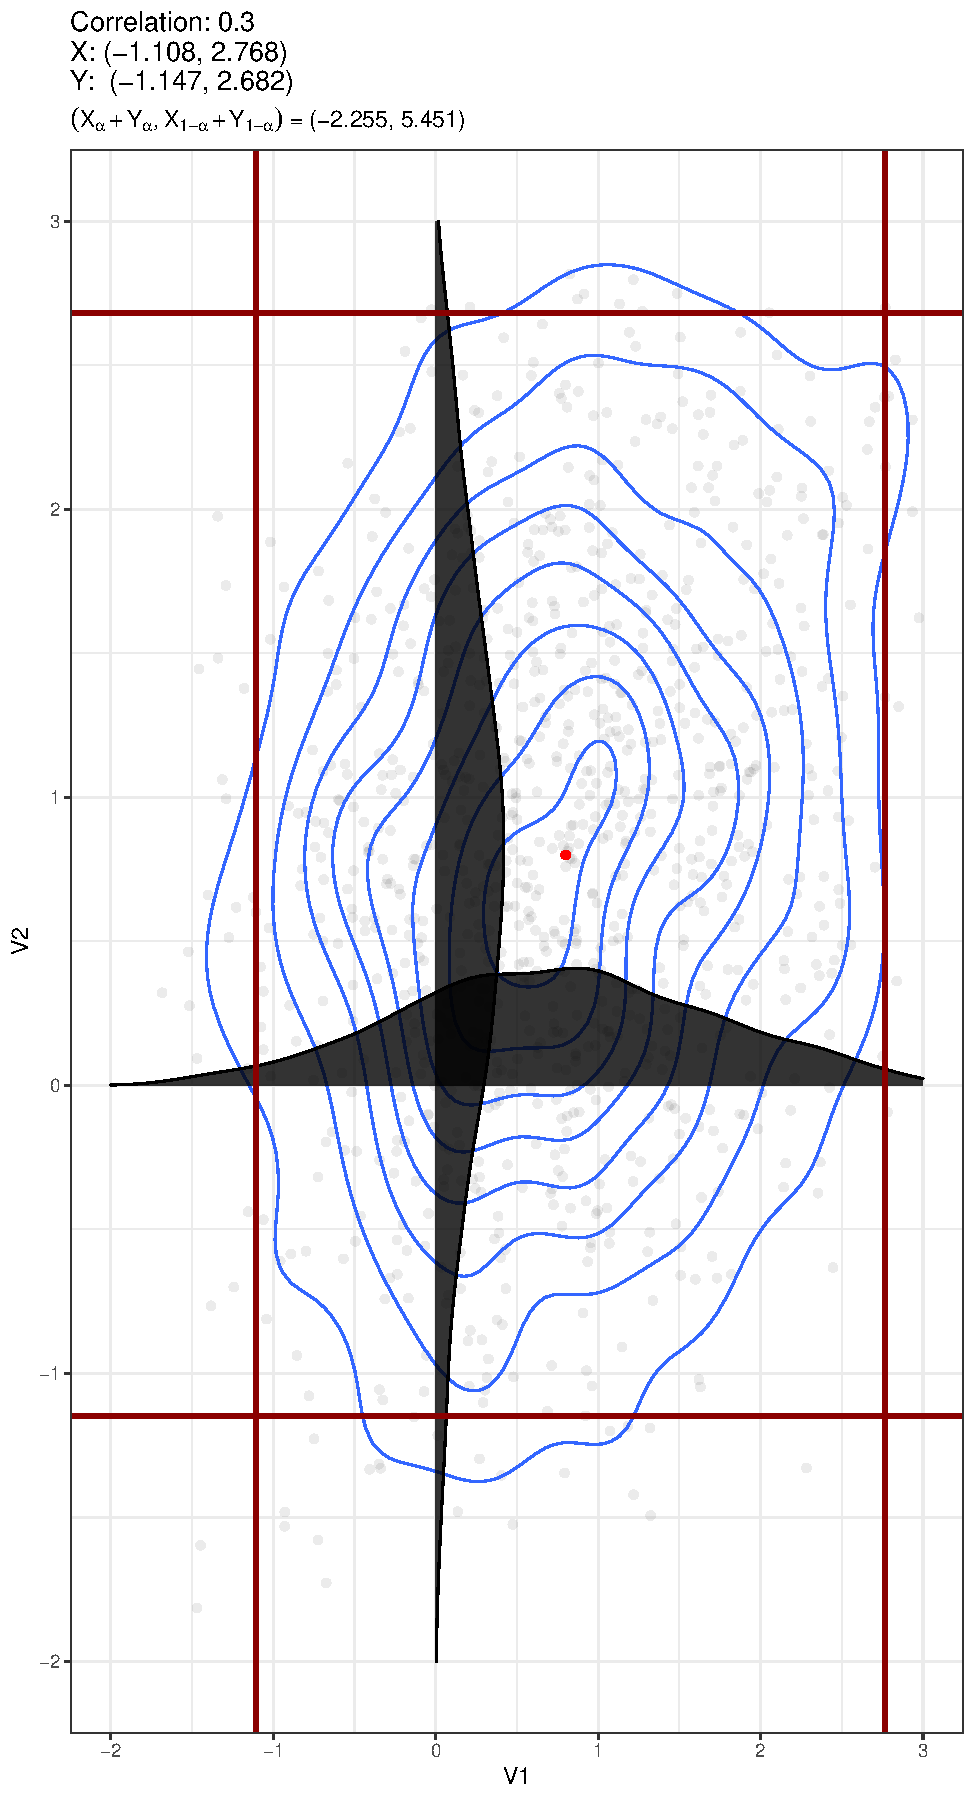
\includegraphics[width=0.96\linewidth]{thesis_files/figure-latex/unnamed-chunk-2-5} 

}

\caption{\label{fig:simmvn}}\label{fig:unnamed-chunk-2}
\end{figure}
In Figure \ref{fig:comp-intervals}, we compare the intervals defined by taking the quantiles of the sum, \(\Big((X+Y)_\alpha, (X+Y)_{1-\alpha}\Big)\), to the intervals taken by summing the quantiles individually, \(\Big(X_\alpha +Y_\alpha, \; X_{1-\alpha} +Y_{1-\alpha}\Big)\). We notice that, as we saw in Figure \ref{fig:simmvn}, increasing the correlation increases the width of the interval \(\Big((X+Y)_\alpha, (X+Y)_{1-\alpha}\Big)\), while the interval \(\Big(X_\alpha +Y_\alpha, \; X_{1-\alpha} +Y_{1-\alpha}\Big)\) is constant since changing the correlation does not change the marginal quantiles \(X_\alpha, X_{1-\alpha}\).,
\begin{figure}

{\centering 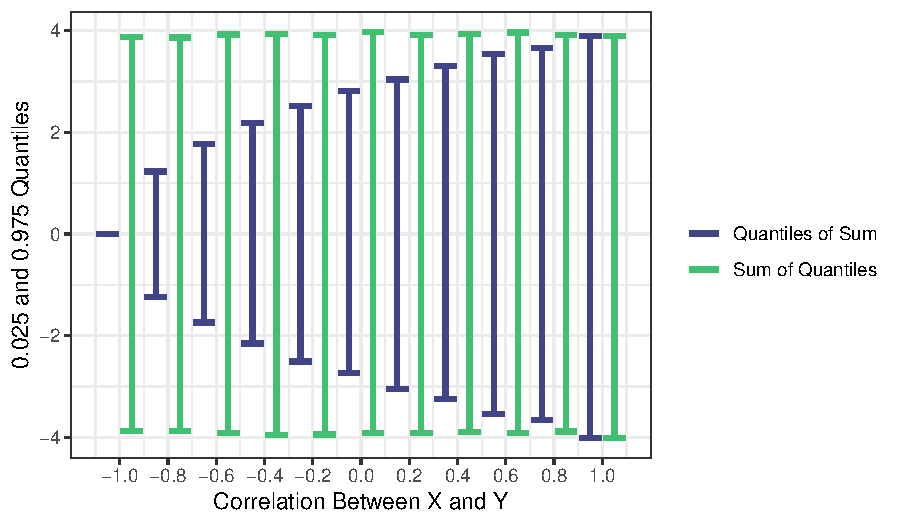
\includegraphics{thesis_files/figure-latex/unnamed-chunk-3-1} 

}

\caption{\label{fig:comp-intervals}}\label{fig:unnamed-chunk-3}
\end{figure}
As we see in Figure \ref{fig:comp-intervals}, the intervals are identical when \(X,Y\) are perfectly correlated. This result is not dependent on the choice of distribution, as we can show by considering CDFs and quantile functions of a general distribution.
\begin{tcolorbox}[title = Quantiles of the Sum of Perfectly Correlated Random Variables]
When two random variables $X$ and $Y$ are perfectly correlated,
$$X_\alpha + Y_\alpha = (X+Y)_\alpha.$$
\end{tcolorbox}
When \(X\) and \(Y\) are perfectly correlated, \(Y\) must be a linear combination of \(X\), so we can write \(X+Y= X+bX=(1+b)X\).

Then, let the \(\alpha^{th}\) quantile of \((1+b)X\) be \(x_\alpha\). By definition of the quantile function, we have

\[F^{-1}_{(1+b) X } (\alpha) = x_\alpha \implies P((1+b) X \leq x_\alpha) = \alpha.\]
Since \((1+b)\) is just a constant, we can divide to yield

\[P\Big( X \leq x_\alpha/(1+b) \Big) = \alpha.\]
To optain hte quantile for \(bX\), we can multiply each side by \(b\) to yield
\[P\Big( bX \leq bx_\alpha/(1+b) \Big) = \alpha.\]
Putting these results together, we have
\begin{align*}
F^{-1}_{bX} (\alpha) + F^{-1}_{X} (\alpha) = \frac{bx_\alpha } { 1+b} + \frac{x_\alpha}{1+b}
&= x_\alpha 
&= F^{-1}_{(1+b)X}(\alpha) \end{align*}

\hypertarget{derivation-of-the-distribution-of-xy-for-bivariate-normal}{%
\subsection{Derivation of the Distribution of X+Y for Bivariate Normal}\label{derivation-of-the-distribution-of-xy-for-bivariate-normal}}

We can see why we observe this relationship between intervals based on the the sum of the \(\alpha^{th}\) quantiles of the individual distributions, \(X_\alpha + Y_\alpha\), and the intervals based on the \(\alpha^{th}\) quantile of the distribution of \(X+Y\) by considering the definition of the quantile function of the normal distribution.

Defining \(Z=g(X,Y) = X+Y\), we can obtain the density function by a change of variables. Notice if \(g(X,Y) = X+Y\), \(g^{-1}(X,Z) = Z-X\), so we have
\begin{align*} f_{X,Z}(x,z) &= f_{X,Y}(x,g^{-1}(x,z)) \left|\frac{\partial g^{-1}(x,z)}{\partial z}\right| \\
f_{X,Z}(x,z) &= f_{X,Y}(x,z-x) \left|\frac{\partial (x-z)}{\partial z}\right|\\
f_{X,Z}(x,z) &= f_{X,Y}(x,z-x) \left|1\right|\\
f_{X,Z}(x,z) &= f_{X,Y}(x,z-x) \\
\end{align*}
Then, we can marginalize out \(X\) to get the PDF of \(f_Z\) by taking

\[f_Z(z) = \int_{\infty}^\infty f(x,z-x) \; dx.\]

Since \((X,Y)\) is bivariate normal with correlation \(\rho\), the PDF is given by

\[f(x,y) = \dfrac{exp\left[\dfrac{-1}{2(1-\rho^2)} \left( \dfrac{(x-\bar x)^2}{\sigma_x^2}+\dfrac{(y-\bar y)^2}{\sigma_x^2} - \dfrac{2 \rho (x-\bar x)(y-\bar y)}{\sigma_x\sigma_y} \right)\right]}{2\pi \sigma_x \sigma_y \sqrt{1- \rho^2}}\]

Integrating with respect to \(x\)\footnote{This integration is extremely long and technical, so we do not include it here.}, we have

\[f_Z(z)  = \int_{-\infty}^\infty \dfrac{\exp\left[\dfrac{-1}{2(1-\rho^2)} \left( \dfrac{(x-\bar x)^2}{\sigma_x^2}+\dfrac{(y-\bar y)^2}{\sigma_x^2} - \dfrac{2 \rho (x-\bar x)(z-x-\bar y)}{\sigma_x\sigma_y} \right)\right]}{2\pi \sigma_x \sigma_y \sqrt{1- \rho^2}} dx \]
\[=\dfrac{\exp\left[-\dfrac{(z-(\bar x + \bar y ))^2}{2(\sigma^2_x+\sigma^2_y + 2\rho \sigma_x \sigma_y)}\right]}{\sqrt{2\pi(\sigma_x^2 + \sigma_y^2 + 2\rho \sigma_x \sigma_y)}}.\]
It follows that \(Z\) is a normal random variable with mean \(\bar x + \bar y\) and standard deviation \(\sqrt{\sigma_x^2 +\sigma_y^2 + 2 \rho \sigma_x \sigma_y }\).

In Figure \ref{fig:ex-sim-normal}, we plot the density estimate of the distribution of \(X+Y\) for \((X,Y) \sim MVN\left( \begin{pmatrix} 0\\0 \end{pmatrix}, \begin{pmatrix} 1 & 0.2 \\0.2 & 1 \end{pmatrix}\right)\) and plot the density of the random variable \(X+Y = Z \sim N\left(\bar x + \bar y,\sqrt{\sigma_x^2 +\sigma_y^2 + 2 \rho \sigma_x \sigma_y }\right)\) and see they are in close alignment, as expected.
\begin{figure}

{\centering 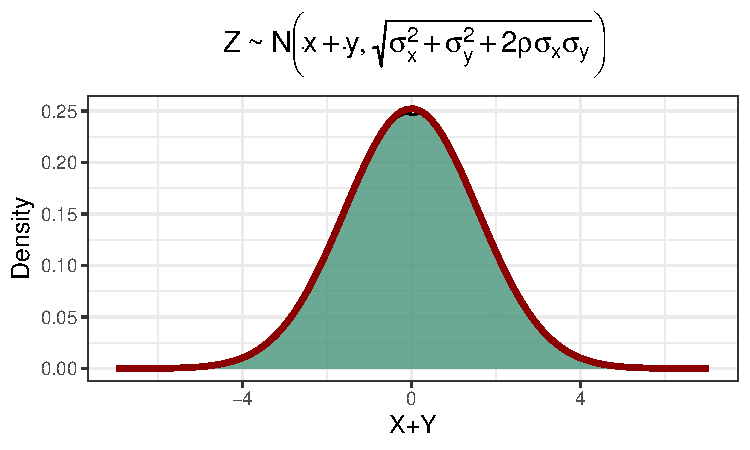
\includegraphics{thesis_files/figure-latex/unnamed-chunk-6-1} 

}

\caption{\label{fig:ex-sim-normal} The theoretical density of $N\left(\bar x + \bar y,\sqrt{\sigma_x^2 +\sigma_y^2 + 2 \rho \sigma_x \sigma_y }\right)$ is plotted in red over the kernel density estimate of the observed distribution of $X+Y$.}\label{fig:unnamed-chunk-6}
\end{figure}
Since we now know \(Z \sim N\left(\bar x + \bar y,\sqrt{\sigma_x^2 +\sigma_y^2 + 2 \rho \sigma_x \sigma_y }\right)\), we can consider the quantile function of the normal distribution, which is defined as

\[F_Z^{-1}(\alpha)=\mu +\sigma_Z \; \text{erf}^{-1}(2\alpha - 1).\]
and since \(\sigma_Z=\sqrt{\sigma_x^2 +\sigma_y^2 + 2 \rho \sigma_x \sigma_y }\) we have
\[F_Z^{-1}(\alpha)=\mu + \left(\sqrt{\sigma_x^2 +\sigma_y^2 + 2 \rho \sigma_x \sigma_y } \right) \; \text{erf}^{-1}(2\alpha - 1).\]
Now, we note the inverse error function \(\text{erf}^{-1}\) is increasing (Figure \ref{fig:erf}).

This means if \(\alpha > 0.5\), \(F_Z^{-1}\) is increasing with increasing values of \(\rho\), and if \(\alpha < 0.5\), \(F_Z^{-1}\) is decreasing with increasing values of \(\rho\).

This if we have a pair of correlated random variables \((X_1,Y_1)\) and \((X_2,Y_2)\) and \(\rho_{X_1,Y_1} > \rho_{X_2,Y_2}\) and consider \(\alpha < 0.5\),

\[(X_1+Y_1)_\alpha <(X_2+Y_2)_\alpha\]

and

\[(X_1+Y_1)_{1-\alpha} > (X_2+Y_2)_{1-\alpha}.\]
This is exactly what we observed in Figure \ref{fig:comp-intervals}.
\begin{figure}

{\centering 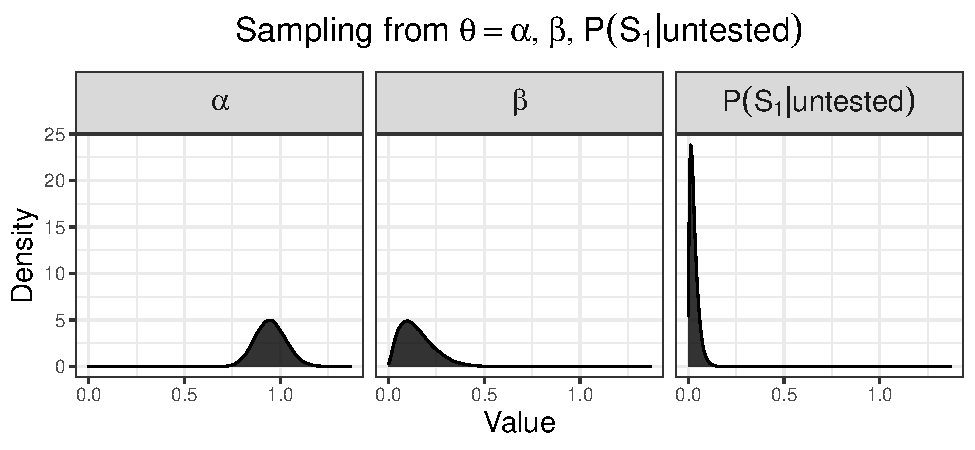
\includegraphics{thesis_files/figure-latex/unnamed-chunk-7-1} 

}

\caption{\label{fig:erf}}\label{fig:unnamed-chunk-7}
\end{figure}
\hypertarget{references}{%
\chapter*{References}\label{references}}
\addcontentsline{toc}{chapter}{References}

Placeholder


% Index?

\end{document}
